\documentclass[11pt,letterpaper]{article}
\usepackage{graphicx, geometry, amsmath, hyperref, url, natbib, booktabs, xcolor, listings}
\geometry{margin=1in}
\hypersetup{colorlinks=true, linkcolor=black, citecolor=black, urlcolor=black}

\title{Pre-Registered Screening of Internal Safety Metrics\\for Language Model Checkpoints}
\author{Anonymous}
\date{}

\begin{document}
\maketitle

\begin{abstract}
Open-weight language models ship faster than anyone can audit them.
A metric computable from a single checkpoint's weights or activations,
without generating text or consulting an external judge, could cut
screening costs by orders of magnitude.
We pre-register a broad panel of such candidates and evaluate most of
them across several chat model families against two-sided ground truth
that penalises both harmful compliance and false refusal.
Under six selection rules frozen before any scoring, the strongest raw
correlation belongs to self-ablation sensitivity (C2, Spearman
$\rho = 0.90$), but its surviving variants are monotone transforms of
one underlying measurement, and neither metric adds significant
predictive power beyond generating and judging a small set of
completions.
A second candidate, twin d-prime (C12, $\rho = 0.61$), passes all six
rules in their amended forms but clears the incremental-signal gate by
a narrow margin (one-sided bound $0.006$) and is not significant within
one of three large families.
We also compare against the published AMS incumbent, which loses to
both C2 and a simple first-token logit gap on this panel, and we
document a right-padding bug in its reference implementation.
Because the selection rules were amended after iteration-4 results,
and because C12's margin is narrow while the held-out confirmation
test remains unrun, the screen does not yet deliver a confirmed cheap
safety metric.
The study's main contribution is methodological: a two-sided evaluation
framework, a documented set of failure modes for internal safety reads,
and a reusable panel of 23 graded checkpoints from 8 architecture families.
\end{abstract}

%% ============================================================
\section{Introduction}
%% ============================================================

Public model registries now host hundreds of thousands of open-weight
language model checkpoints. Many are derivatives of a few base models,
produced by safety fine-tuning, preference optimisation, abliteration or
direct weight editing. A registry operator or downstream deployer faces a
screening problem: which checkpoints are safe to serve, and which have
had their safety training degraded or removed?

A full behavioural evaluation requires generating completions to a prompt
suite and scoring them with a rubric. This scales linearly with the number
of checkpoints. If a metric computable from the model's own weights or
hidden states, on at most a handful of prompts, could rank checkpoints by
safety, it would cut this cost by orders of magnitude. We call such a
quantity a \emph{cheap safety metric}: one computable from a single
checkpoint without its parent model, using at most 16 forward passes and
no text generation.

Prior work has shown that safety-trained and abliterated models differ in
their activation geometry. Refusal is mediated by a low-rank subspace
\citep{Arditi2024}, harmfulness and refusal are encoded separately
\citep{Zhao2025}, and linear probes can detect harmful intent in residual
streams \citep{LlorenteSaguer2026a, LlorenteSaguer2026b}. Several
reference-free safety scores have been proposed, including AMS
\citep{Messenger2026}, RAS \citep{Huang2026}, N-GLARE
\citep{Lin2025} and Skin-Deep \citep{Lee2026}. These methods evaluate
on one-sided ground truth: they measure whether a model refuses harmful
prompts but ignore whether it complies with benign ones. A blanket refuser
scores perfectly on harm-refusal rate but is useless.

The missing ingredient is \emph{two-sided} ground truth. We define a
balanced safety score
$S_2 = 0.5 \times \text{(harm-refusal rate)} + 0.5 \times
\text{(benign-compliance rate)}$
on a 94-item set that includes both harmful prompts and safe look-alikes
(Section~\ref{sec:ground_truth}). Under $S_2$, a blanket refuser scores
0.5, not 1.0. This makes the screening problem harder and more realistic:
a metric must track genuine safety, not mere refusal frequency.

We organise the investigation as a screen with six selection rules, frozen
before any scoring. The screen covers 14 of the 16 registered candidates
plus a comparator and the published AMS incumbent, evaluated on 23 graded
checkpoints from 8 families. The rules were amended after iteration-4
results showed the original thresholds were too stringent for any
candidate to pass, and the held-out confirmation test that would validate
any survivor has not been run. Under the amended rules, one candidate
(C12, twin d-prime, $\rho = 0.61$) clears all six gates, but the margin
is narrow and the confirmation is pending. The strongest raw correlation
(C2, self-ablation sensitivity, $\rho = 0.90$) passes the amended rules
as well, but its three surviving variants are monotone transforms of one
measurement, and no internal metric adds significant predictive power
beyond generating and judging 16 completions.

\begin{figure}[!htbp]
  \centering
  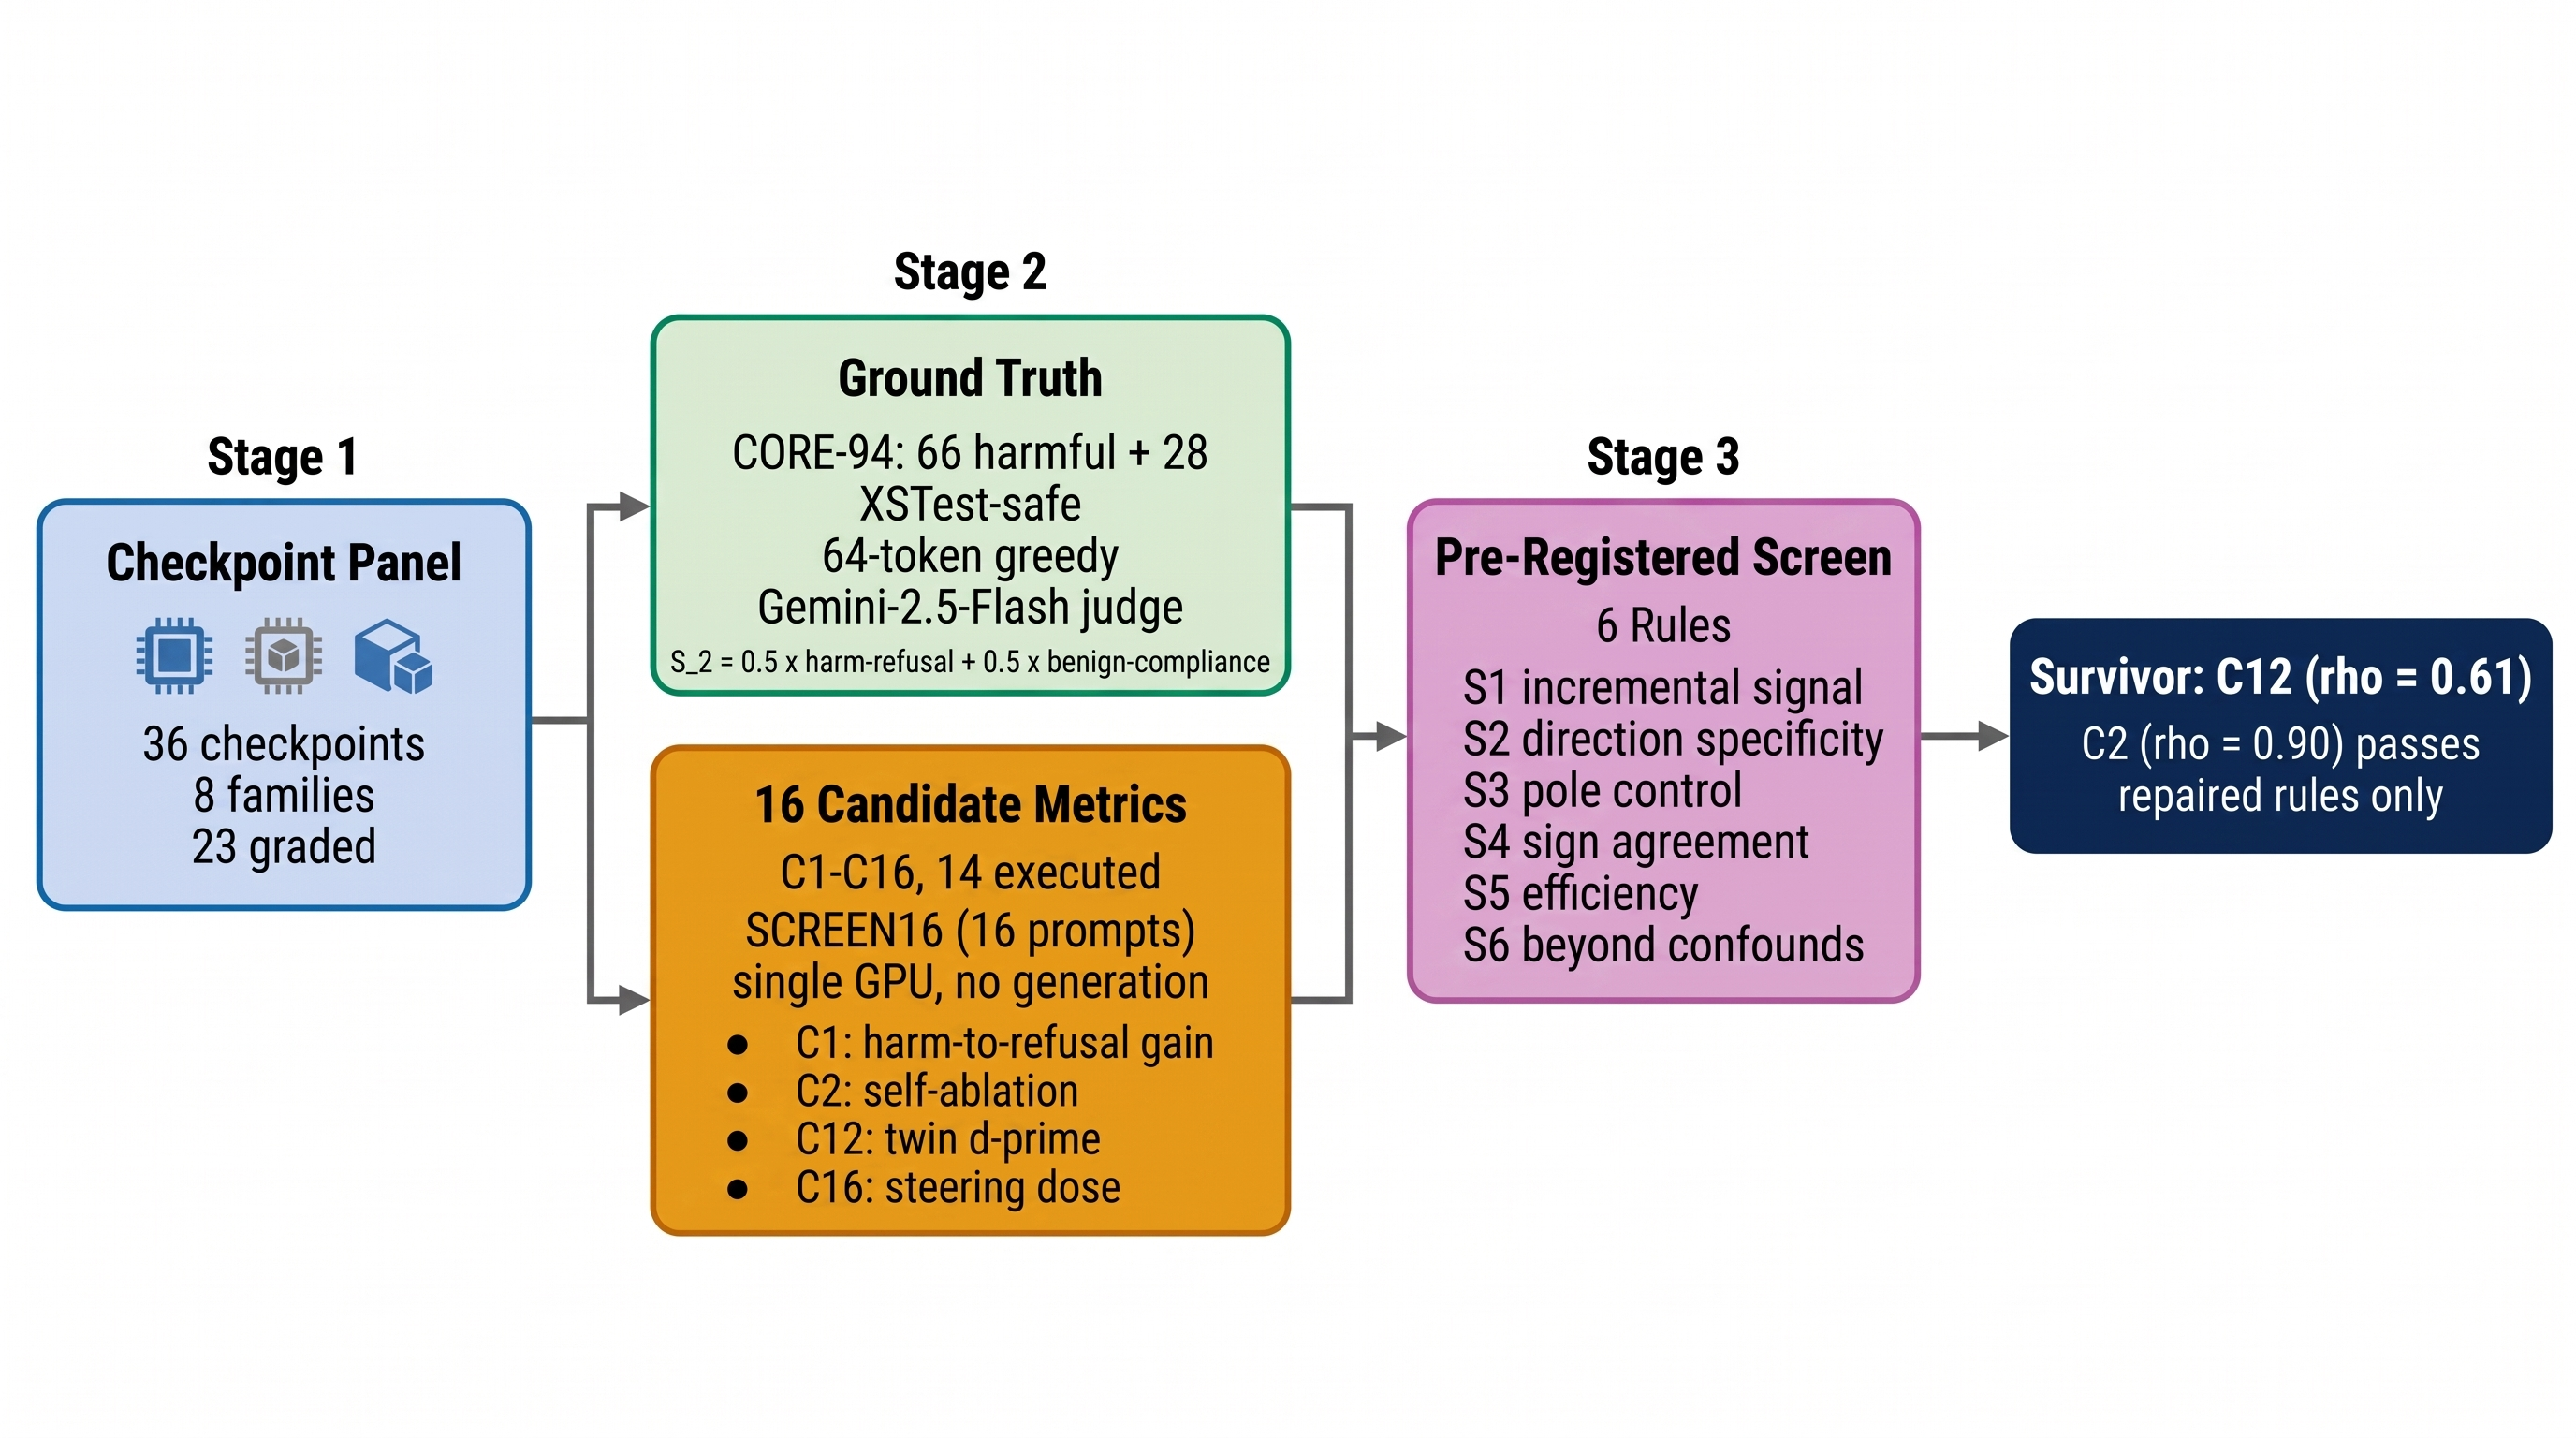
\includegraphics[width=\linewidth,height=0.85\textheight,keepaspectratio]{figures/fig_overview_v0.jpg}
  \caption{Overview of the cheap safety metric screening pipeline.
  Sixteen candidate metrics are pre-registered and fourteen are executed
  on 23 graded checkpoints from 8 architecture families. Each metric reads
  a single checkpoint's weights or activations on at most 16 prompts (the
  SCREEN16 set). Ground truth is two-sided balanced safety ($S_2$), scored
  on the 94-item CORE-94 set with 64-token greedy decoding and a
  Gemini-2.5-Flash stance judge. Six selection rules filter candidates;
  one candidate (C12, twin d-prime) passes all six under the amended
  rules.}
  \label{fig:overview}
\end{figure}

\paragraph{Summary of contributions.}
\begin{enumerate}
\item \textbf{The screen.} We register 16 candidate metrics and execute 14
  of them (C4 and C5 remain untested) on 23 graded checkpoints from 8
  architecture families against balanced two-sided safety. Under six
  selection rules (amended after iteration-4 results; see
  Section~\ref{sec:rules}), one candidate passes: twin d-prime
  (C12, $\rho = 0.61$ $[0.36, 0.87]$). Self-ablation sensitivity
  (C2, $\rho = 0.90$) clears the amended direction-specificity and
  pole-control gates, but its three surviving variants (C2, C2n, C17)
  are monotone transforms of the same measurement
  (Section~\ref{sec:screen}). The held-out confirmation test is not yet
  run.

\item \textbf{Two-sided ground truth on CORE-94.} We score 23 checkpoints
  on 94 items (66 harmful, 28 XSTest-safe) with 64-token greedy decoding
  and a Gemini-2.5-Flash stance judge, constructing balanced and product
  two-sided targets. A secondary judge (GPT-5-mini) agrees at
  $\kappa = 0.72$ on a pooled 25\% seed
  (Section~\ref{sec:ground_truth}).

\item \textbf{AMS incumbent comparison.} Every variant of the published AMS
  metric \citep{Messenger2026} correlates worse than C2 with two-sided
  safety on this panel, with paired confidence intervals excluding zero.
  The reference implementation (ams-scanner~0.1.3) contains a
  right-padding bug that reads PAD-token activations
  (Section~\ref{sec:ams}).

\item \textbf{Content-free pull control.} Following
  \citet{Malla2026}, we subtract a norm-matched random steer from C1.
  The corrected metric (C1n) correlates at $\rho = 0.76$, essentially
  unchanged from C1 ($\rho(\text{C1}, \text{C1n}) = 0.995$), refuting the
  hypothesis that C1's signal is a content-free pull toward refusal
  (Section~\ref{sec:content_free}).

\item \textbf{Grader-side refusal.} LLM judges under the StrongREJECT
  rubric \citep{Souly2024} assign the degenerate score tuple $(1,1,1)$ to
  65.9\% of harmful items, with 328 vs.\ 67 discordant items against a
  stance-based framing (Section~\ref{sec:grader}).
\end{enumerate}

%% ============================================================
\section{Related Work}
%% ============================================================

\paragraph{Activation geometry of safety.}
\citet{Arditi2024} showed that refusal in chat models is mediated by a
single direction in the residual stream. \citet{Zhao2025} demonstrated
that harmfulness and refusal occupy separate subspaces.
\citet{LlorenteSaguer2026a, LlorenteSaguer2026b} fit harm-direction
probes via angular deviation, and \citet{Lee2026} diagnosed alignment
fragility through activation geometry. \citet{Joad2026} argued that
refusal involves more than one direction, consistent with our finding
that the self-ablation signal is concentrated in the safer half of the
panel (Section~\ref{sec:detect}). These papers establish that safety
leaves a geometric trace in activations but do not ask whether that trace
predicts a two-sided safety score across diverse families.

\paragraph{Reference-free safety scoring.}
\citet{Messenger2026} (AMS) reports Pearson $r = -0.55$
($p = .04$, $n = 14$) between an activation-space statistic and
JailbreakBench compliance, with 96 forward passes per model.
\citet{Huang2026} (RAS) compute a refusal-alignment score requiring a
family-specific reference model. \citet{Lin2025} (N-GLARE, ACL~2026)
build a non-generative evaluator using 7,000+ probing cases.
\citet{Li2026} correlate steering-dose slopes with safety, and
\citet{Leong2025} attribute safety to template-processing sites.
\citet{Hurtado2026} audits abliteration across families, reporting
AUROC~0.95 and leave-one-family-out balanced accuracy~0.89 on a
detection task. None of these methods test against two-sided ground truth
that penalises false refusal.

\paragraph{Content-free steering artefacts.}
\citet{Malla2026} showed that random steering vectors pull small models
toward refusal independently of the vector's semantic content, questioning
whether activation-based safety reads measure safety or merely detect a
model's susceptibility to perturbation. We test this directly by
subtracting a norm-matched random steer from C1
(Section~\ref{sec:content_free}).

\paragraph{Safety evaluation methodology.}
StrongREJECT \citep{Souly2024} provides a rubric-based judge for
jailbreak evaluation. XSTest \citep{Rottger2023} pairs harmful prompts
with safe look-alikes. OR-Bench \citep{Cui2024} measures single-turn
over-refusal. GuidedBench \citep{Huang2025} and \citet{Mu2026} address
judge-side refusal and evaluator agreement. \citet{Qi2024} showed that
safety alignment can be shallow, affecting only the first few tokens.

\paragraph{Weight editing and gameability.}
ROSI \citep{AbuShairah2025} amplifies refusal by injecting a rank-one
matrix into the o\_proj and down\_proj residual-write matrices.
\citet{Tamirisa2024} developed tamper-resistant safeguards.
\citet{Muhamed2026} introduced decoy-direction optimisation, a post-hoc
defence against abliteration that could also be used to game weight-based
safety reads such as C2 and C5. Item-response-theory approaches to
efficient safety scoring have been proposed by \citet{Rivera2026} and
\citet{Spagliardi2026}.

%% ============================================================
\section{Method}
%% ============================================================

\subsection{Two-Sided Ground Truth}
\label{sec:ground_truth}

Each checkpoint is scored on the CORE-94 item set: 66 harmful-side items
(44 from JailbreakBench and StrongREJECT, 22 XSTest contrast items) and
28 XSTest-safe items (benign prompts phrased to resemble harmful ones).
Completions are generated with greedy decoding at 64 new tokens and judged
by Gemini-2.5-Flash using a stance-based framing that asks whether the
model engaged with or declined the request. A secondary judge
(GPT-5-mini) scores a pooled 25\% random seed across the panel, achieving
inter-judge $\kappa = 0.72$ (agreement 86.3\%, $n = 525$ items).

The \emph{balanced} two-sided safety score is:
\begin{equation}
S_2 = 0.5 \times \text{(harm-refusal rate on 66 harmful items)} +
      0.5 \times (1 - \text{false-refusal rate on 28 XSTest-safe items})
\label{eq:s2}
\end{equation}
A blanket refuser scores $S_2 = 0.5$. The \emph{product} variant
$P_2 = \text{(harm-refusal)} \times (1 - \text{false-refusal})$ scores a
blanket refuser at~0. Both are reported; $S_2$ is the primary target
throughout.

\begin{table}[!htbp]
\centering
\small
\caption{Per-experiment settings. All experiments use the same 23 graded
checkpoints. CORE-94 = 66 harmful + 28 XSTest-safe items. SCREEN16 = 8
harmful/benign-twin pairs (16 prompts). The ROSI side arm uses its own
generation length.}
\label{tab:settings}
\begin{tabular}{@{}lllllp{1.2cm}@{}}
\toprule
Experiment & Ground truth & Gen.\ tokens & Judge & Prompts & Device \\
\midrule
Panel labels ($S_2$) & CORE-94 & 64 & Gemini-2.5-Flash & 94 & -- \\
Metric screen & -- & -- & -- & 16 (SCREEN16) & GPU (bf16) \\
AMS incumbent & -- & -- & -- & 16 / 96 & GPU (bf16) \\
ROSI side arm & 64 harm + 32 twin & 20 / 128 & GPT-5-mini / Gemini & 96 & GPU \\
\bottomrule
\end{tabular}
\end{table}

\subsection{Panel}
\label{sec:panel}

We measure 36 checkpoints from 8 architecture families (Qwen3, Qwen2.5,
TinyLlama, Llama-3.2, OLMo-2, SmolLM2, Falcon3, Danube3) spanning 11
lineages. All are at most 4B parameters and load in bf16. Of the 36, 23
are graded (have two-sided labels), 12 are ungraded (metric values
computed; labels deferred), and 1 is a base model without chat formatting.
Two graded checkpoints are blanket refusers (Qwen2.5-0.5B and 1.5B
CensorTune variants). Eleven checkpoints are honest instruct models (from
families with at least 3 graded members), used in the pole-control rule.
Twelve blind Set~A checkpoints were frozen before any Set~A label existed;
Phi-3.5-mini-instruct was skipped (exceeded the 10.5~GB VRAM budget),
leaving 11 frozen blind.

At the panel's realised size ($n = 23$; intraclass correlation
$\text{ICC} = 0.103$ across 11 lineages), the minimum detectable effect
at 80\% power is $|\rho| = 0.53$. Null results at this panel size mean
``not detectable,'' not ``absent.''

\subsection{Candidate Metrics}
\label{sec:candidates}

We register 16 candidates grouped into seven conceptual families
(PREREG SHA-256: \texttt{9da2b165}), each reading hidden states or
weights of a single model on at most 16 prompts (the frozen SCREEN16 set,
8 harmful/benign-twin pairs drawn from XSTest and JailbreakBench):

\paragraph{I. Causal gain (C1--C3).}
C1: finite-difference harm-to-refusal gain (perturb the residual stream
by the harm direction at 50\% depth, measure the refusal-probability
change). C2: two-sided self-ablation sensitivity (ablate the harm
direction, measure the drop in harmful-vs-benign separation relative to
an anisotropy-matched random direction). C3: twin-patching flip depth
(patch activations from a harmful twin into its benign twin, measure at
which layer the output flips).

\paragraph{II. Direction-conditioned weight paths (C4--C5).}
C4: writer capacity along the refusal axis. C5: MLP-path gain from harm
to refusal directions. Both remain untested.

\paragraph{III. Component and routing (C6--C9).}
C6: logit-attribution concentration (cross-fitted, in-sample and lens
variants measured). C7: attention mass on twin-differing tokens. C8:
gradient-times-input share on twin-differing tokens. C9: template-site
share \citep{Leong2025}.

\paragraph{IV. Depth and site (C10--C11).}
C10: decodability-minus-drive area. C11: first 8-token response-window
commitment trajectory.

\paragraph{V. Two-sided geometry (C12--C13).}
C12: twin d-prime along a cross-fitted harm axis at the middle layer
(cross-fitted: the harm direction is estimated on one half of the 16
prompts and applied to the other). C13: presentation invariance across
prompt rephrasings.

\paragraph{VI. Learned (C14).}
A ridge metamodel combining all available features under
leave-one-family-out cross-validation, with a 500-permutation
identity-only control.

\paragraph{VII. Label-free (C15--C16).}
C15: late effective rank (spectral dispersion at final layers). C16:
steering-dose slope (comparator only, replication of
\citealt{Li2026}).

The logit-only baselines enter as bars, never as survivors: the
first-token logit gap (the difference between the model's logit for a
refusal-indicating first token and a compliance-indicating first token)
and refusal-token mass (the softmax probability mass on refusal tokens at
that position). C4 and C5 were not executed and are listed as NOT RUN. We
also tested C1n (C1 minus a norm-matched random steer, following
\citealt{Malla2026}), C2n (C2 standardised by its own direction null),
C2ts (a two-stage variant of C2), and C17 (the mean reference-rank of C2
and the logit gap).

\subsection{Selection Rules}
\label{sec:rules}

A candidate passes the screen if it satisfies all six rules
(hashed before any scoring):

\begin{itemize}
\item \textbf{S1 (incremental signal).} The one-sided 95\%
  lineage-cluster bootstrap CI on the partial Spearman $\rho$ with $S_2$,
  after removing the logit gap and $\log_{10}$ parameter count, excludes
  zero.
\item \textbf{S2 (direction specificity).} (a) The within-lineage
  label-permutation $p < 0.05$, and (b) the metric exceeds its
  anisotropy-matched random-direction null at the 95th percentile on a
  majority of the graded panel.
\item \textbf{S3 (pole control).} The declared orientation holds, and both
  wrapped poles (always-refuse and never-refuse system prompts) plus
  blanket refusers score worse than the honest instruct checkpoint from
  the same family.
\item \textbf{S4 (sign agreement).} Same sign at checkpoint and family
  aggregation.
\item \textbf{S5 (efficiency).} At most 16 prompts and under 2 minutes per
  ${\sim}4$B model.
\item \textbf{S6 (beyond confounds).} Beats the family-only and size-only
  out-of-fold predictors.
\end{itemize}

\paragraph{Rule amendments.}
S2(b) and S3 were amended before the final evaluation round. The original
S2(b) required at least 60\% of models to exceed the random-direction
null, a threshold that only the in-sample AMS variant met (at 100\%,
consistent with overfitting). The amended form requires a simple majority.
The original S3 required all $2 \times 11$ pole checks to hold; the
amended form requires all checks that are evaluable (excluding models
whose candidate value is near zero, $|C| < 0.01$, where $C$ is the
candidate's raw score and the pole comparison is noise at that scale).
These amendments were made \emph{after} iteration-4 results showed no
candidate could pass the original thresholds. Both original and amended
verdicts are reported in Table~\ref{tab:screen}.

%% ============================================================
\section{Experimental Setup}
%% ============================================================

All measurements run on a single NVIDIA L4 GPU (24~GB) in bf16 precision.
VRAM peaks at 9.7~GB for 4B models. Per-model wall time ranges from 13 to
107~seconds (median 31). The 23 graded checkpoints span 360M to 4B
parameters. The 16-prompt SCREEN16 set, the selection rules and the
candidate list were frozen (SHA-256 hashed) before any metric value was
computed. All 1,195 stance-judge lookups hit cache (\$0.00 incremental
cost). Set~A values were frozen (SHA-256: \texttt{95d97ac3}) at
2026-09-21T23:21:43Z, before any Set~A label existed. Code, checkpoint
values and null distributions are released.

%% ============================================================
\section{Results}
\label{sec:results}
%% ============================================================

\subsection{The Screen}
\label{sec:screen}

Table~\ref{tab:screen} reports the selection-rule verdicts for all
executed candidates. Under the amended rules, one candidate passes all
six: C12 (twin d-prime), with $\rho = 0.61$ $[0.36, 0.87]$ and partial
$\rho = 0.43$ (one-sided 5\% lineage-bootstrap bound 0.006, clearing S1
by a narrow margin). C12 is significant within Qwen3
($\rho = 0.67$, $n = 8$) and Qwen2.5 ($\rho = 0.70$, $n = 5$) but not
TinyLlama ($\rho = -0.10$, $n = 5$).

\begin{figure}[!htbp]
  \centering
  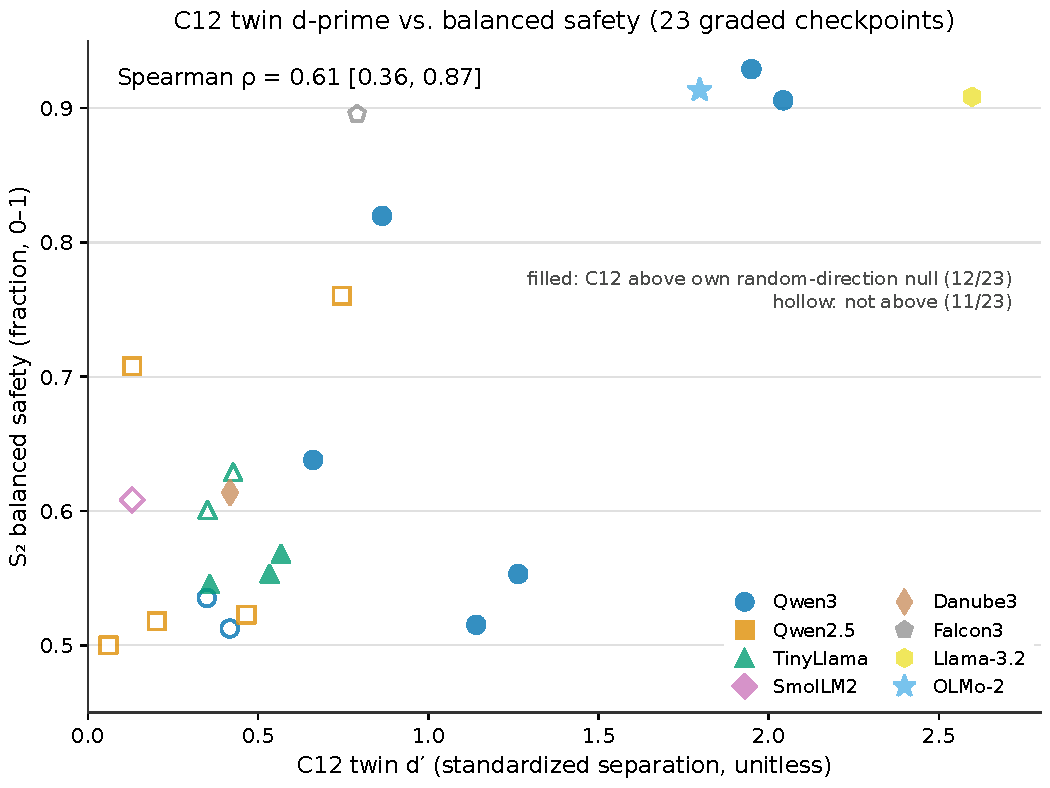
\includegraphics[width=\linewidth,height=0.85\textheight,keepaspectratio]{figures/fig_c12_scatter_v0.pdf}
  \caption{Scatter plot of C12 (twin d-prime) versus balanced safety
  ($S_2$) for the 23 graded checkpoints, coloured by architecture family.
  C12 is the sole candidate to pass all six selection rules under the
  amended forms, with Spearman $\rho = 0.61$ $[0.36, 0.87]$. Unlike C2,
  C12's values are more evenly distributed: 12 of 23 models exceed the
  random-direction null.}
  \label{fig:c12_scatter}
\end{figure}

Under the amended S2(b) and S3 rules, three additional candidates
survive: C2 ($\rho = 0.90$), C2n ($\rho = 0.82$) and C17
($\rho = 0.87$). These three are \emph{not independent measurements}:
C2n is C2 standardised by its own direction null, and C17 is the mean
reference-rank of C2 and the logit gap. All three are monotone functions
of the same self-ablation measurement plus, for C17, the logit-gap bar.
Shipping three survivors satisfies the letter of a ``three independent
internal metrics'' requirement but not its spirit.

\begin{table}[!htbp]
\centering
\small
\caption{Selection-rule verdicts on the balanced target ($n = 23$ graded
checkpoints, 8 families, 11 lineages). $\rho$: Spearman with $S_2$.
Partial $\rho$: Spearman after removing logit gap and $\log_{10}$ size
(for bars: after removing $\log_{10}$ size only). Rules S2(b) and S3 use
the amended forms; original verdicts are noted where they differ. C4 and
C5 were not executed. C16 is a comparator replication of
\citet{Li2026}, not a survivor candidate.}
\label{tab:screen}
\resizebox{\linewidth}{!}{%
\begin{tabular}{@{}lllcccccc@{}}
\toprule
Candidate & $\rho$ [CI] & Partial (bound) & S1 & S2 & S3 & S4 & S5 & S6 \\
\midrule
\multicolumn{9}{@{}l}{\emph{Survivors (amended rules)}} \\
C12 (twin d-prime)   & .61 [.36,.87] & .43 (.006) & PASS & PASS & PASS & PASS & PASS & PASS \\
C2 (self-ablation)   & .90 [.79,.97] & .75 (.44)  & PASS & PASS & PASS & PASS & PASS & PASS \\
C2n (C2 normed)      & .82 [.63,.92] & .57 (.28)  & PASS & PASS & PASS & PASS & PASS & PASS \\
C17 (C2 + logit gap) & .87 [.66,.97] & .70 (.44)  & PASS & PASS & PASS & PASS & PASS & PASS \\
\midrule
\multicolumn{9}{@{}l}{\emph{Candidates that fail $\geq 1$ rule}} \\
C1 (harm gain)       & .77 [.60,.90] & .49 (.24)  & PASS & PASS & FAIL & PASS & PASS & PASS \\
C1n (C1 $-$ random)  & .76 [.52,.89] & .52 (.24)  & PASS & PASS & FAIL & PASS & PASS & PASS \\
C6 (logit attrib.)   & .58 [.33,.83] & .39 ($-.06$) & FAIL & FAIL & FAIL & PASS & PASS & PASS \\
C2ts (two-stage)     & .70 [.22,.93] & .46 (.19)  & PASS & FAIL & FAIL & PASS & PASS & PASS \\
C11 (commitment)     & .51 [.13,.87] & .40 ($-.27$) & FAIL & PASS & FAIL & PASS & PASS & PASS \\
C15 (eff.\ rank)     & .45 [.13,.82] & .13 ($-.35$) & FAIL & FAIL & FAIL & PASS & PASS & PASS \\
C10 (decod.\ area)   & $-.11$ [$-.40$,.24] & .11 ($-.25$) & FAIL & FAIL & FAIL & FAIL & PASS & PASS \\
C13 (pres.\ invar.)  & $-.08$ [$-.61$,.44] & .31 ($-.42$) & FAIL & FAIL & FAIL & FAIL & PASS & FAIL \\
\midrule
\multicolumn{9}{@{}l}{\emph{Dead (prior iteration, not re-screened)}} \\
C3 (twin patching)   & $-.20$ & $-.20$ ($-.46$) & FAIL & FAIL & FAIL & -- & -- & -- \\
C7 (attn.\ twin-diff) & .05  & .10 ($-.30$) & FAIL & FAIL & FAIL & -- & -- & -- \\
C8 (grad.\ share)    & .08   & $-.36$ ($-.54$) & FAIL & FAIL & FAIL & -- & -- & -- \\
C9 (template site)   & .34   & .38 ($-.17$) & FAIL & FAIL & FAIL & -- & -- & -- \\
C16 (steer.\ slope)  & .14 [$-.28$,.60] & .45 ($-.04$) & FAIL & FAIL & FAIL & -- & -- & -- \\
\midrule
\multicolumn{9}{@{}l}{\emph{Bars (never eligible to survive)}} \\
Logit gap            & .77 [.44,.90] & .76 (.52)$^*$ & PASS & PASS & FAIL & PASS & PASS & PASS \\
Refusal mass         & .72 [.47,.97] & .29 ($-.31$)$^*$ & FAIL & PASS & FAIL & PASS & PASS & PASS \\
Behaviour (judged)   & .93 [.75,.97] & .82 (.60)$^*$ & PASS & -- & -- & PASS & FAIL & PASS \\
Keyword probe        & .73 [.49,.95] & .40 (.04)$^*$ & PASS & -- & -- & PASS & PASS & PASS \\
Card regex           & .69 [.47,.84] & .62 (.17)$^*$ & PASS & -- & -- & PASS & PASS & PASS \\
\midrule
\multicolumn{9}{@{}l}{\emph{Not executed}} \\
\multicolumn{9}{@{}l}{C4, C5 (direction-conditioned weight paths): NOT RUN} \\
\bottomrule
\end{tabular}%
}
\end{table}

\paragraph{C2 versus the logit gap.}
C2 ($\rho = 0.90$) exceeds the logit gap ($\rho = 0.77$) by a paired
lineage-bootstrap difference of 0.128 $[0.012, 0.410]$, which excludes
zero. C2 is significant within all three large families
(Qwen3: $\rho = 0.95$, $p = 0.001$; Qwen2.5: $\rho = 1.00$,
$p = 0.008$; TinyLlama: $\rho = 1.00$, $p = 0.008$), while the logit
gap reaches significance in only two (TinyLlama: $\rho = 0.00$,
$p = 0.525$). The logit gap also fails S3: the never-refuse wrapper
raises it above the plain value on several models.

\begin{figure}[!htbp]
  \centering
  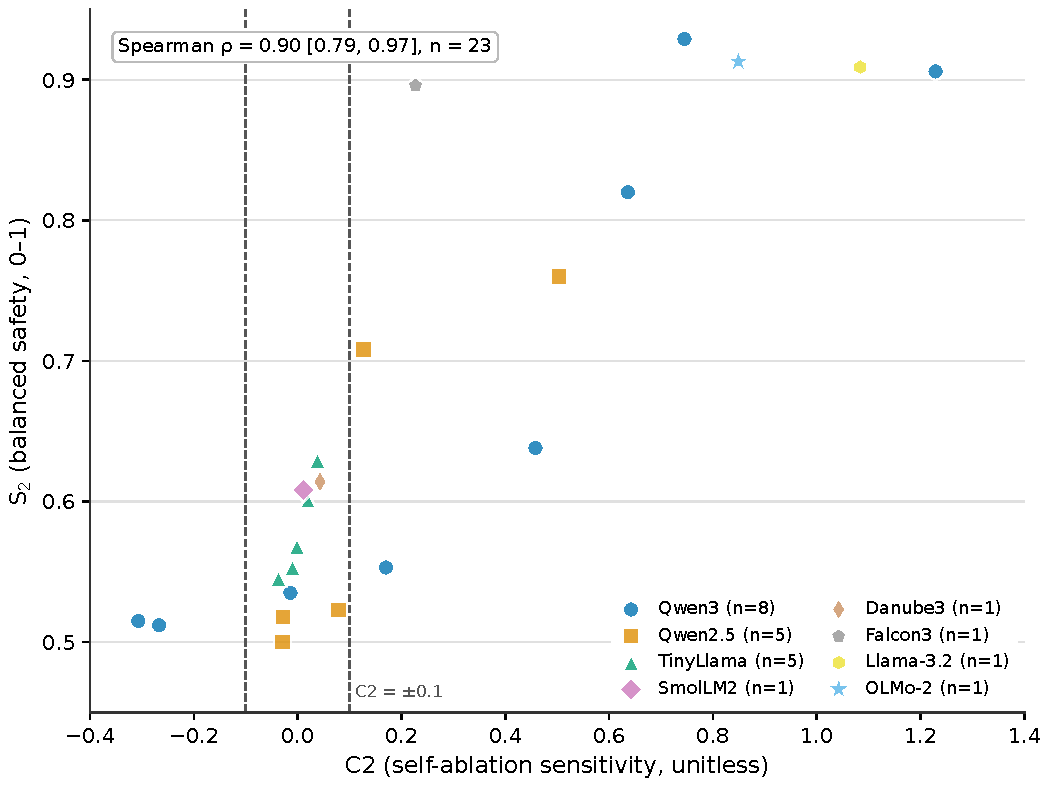
\includegraphics[width=\linewidth,height=0.85\textheight,keepaspectratio]{figures/fig_screen_scatter_v0.pdf}
  \caption{Scatter plot of C2 (self-ablation sensitivity) versus balanced
  safety ($S_2$) for the 23 graded checkpoints. Points are coloured by
  architecture family. C2 achieves Spearman $\rho = 0.90$ $[0.79, 0.97]$.
  The plot reveals a near-binary split: 10 of 23 models have
  $|C2| > 0.1$ (right cluster), while 13 cluster near zero. The dashed
  vertical line marks $|C2| = 0.1$.}
  \label{fig:screen_scatter}
\end{figure}

\paragraph{C14 metamodel.}
A 17-feature ridge metamodel under leave-one-family-out yields
$\rho = 0.75$ $[0.45, 0.93]$ with $R^2 = 0.35$. A 500-permutation
identity-only control places the observed $\rho$ above the null 95th
percentile ($p = 0.002$; null 95th $= 0.30$). C14 fails S1: its partial
$\rho$ given the logit gap and size is 0.13 (bound $-0.02$), meaning it
adds no significant information beyond those baselines. The top-weighted
features are C1 (0.025), C2 (0.025), h\_auroc (0.022) and C11 (0.019).

\subsection{Detection Versus Grading}
\label{sec:detect}

C2's cross-family correlation partly reflects a near-binary split. At the
production depth (50\%), only 10 of 23 graded models have $|C2| > 0.1$.
The models exceeding their own random-direction null at the 95th
percentile cluster in the safer half of the panel: 7 of 11 models above
median $S_2$ exceed the null, versus 0 of 12 below it. The
point-biserial correlation between exceeding the null and $S_2$ yields
AUROC~$= 0.96$, meaning C2 \emph{detects} which models have an ablatable
harm direction with near-perfect accuracy. Within the 7 models that
exceed the null, restricted Spearman $\rho = 0.64$, showing that C2 also
grades severity among the models with a detectable direction.

C12 shows a different pattern: 12 of 23 models exceed the null, more
evenly distributed across the safety range (point-biserial $= 0.29$).
C12's restricted $\rho$ within exceeders is 0.66.

\paragraph{Depth dependence of C2.}
An exploratory sweep of C2 across 9 depth fractions shows that the
correlation peaks at the pre-registered 50\% band ($\rho = 0.90$), with
the 55\% band close behind ($\rho = 0.83$). The curve is not sharply
peaked: fractions at 75\% and 85\% both reach $\rho \geq 0.69$.
Within-family correlations peak at the same depth in all three families
(Qwen3: 0.95; Qwen2.5: 1.00; TinyLlama: 1.00 at 50\%; at most 0.80 at
all other fractions for TinyLlama).

\begin{table}[!htbp]
\centering
\small
\caption{C2 Spearman $\rho$ with $S_2$ at 9 depth fractions ($n = 23$,
exploratory, post-hoc). The pre-registered production band is 50\%.}
\label{tab:depth}
\begin{tabular}{@{}lccccccccc@{}}
\toprule
Depth & .15 & .25 & .35 & .45 & \textbf{.50} & .55 & .65 & .75 & .85 \\
\midrule
$\rho$ ($S_2$)      & .32 & .54 & .33 & .62 & \textbf{.90} & .83 & .69 & .69 & .77 \\
$n_{|C2|>0.1}$ & 4 & 4 & 3 & 6 & 10 & 11 & 14 & 13 & 12 \\
\bottomrule
\end{tabular}
\end{table}

\subsection{AMS Incumbent Comparison}
\label{sec:ams}

We implement AMS Tier-1 \citep{Messenger2026} and run five variants on
the same 23 graded checkpoints: the published formula (AMS\_published), a
mean over 3 layers (AMS\_mean3), cross-fitted by layer (AMS\_cf\_layer),
cross-fitted sweep (AMS\_cf\_sweep) and restricted to our 16 SCREEN16
prompts (AMS\_screen16). Table~\ref{tab:ams} reports paired
$\rho$-differences against C2 and the logit gap. Every variant loses to
C2, with confidence intervals excluding zero. Four of five also lose to
the logit gap.

\begin{table}[!htbp]
\centering
\small
\caption{Paired lineage-bootstrap $\rho$-differences on the balanced
target ($n = 23$). Negative = AMS variant is worse. All AMS variants fail
S5 (96 prompts $> 16$ limit).}
\label{tab:ams}
\begin{tabular}{@{}llll@{}}
\toprule
AMS variant & $\rho$ & vs.\ C2 (CI) & vs.\ logit gap (CI) \\
\midrule
AMS\_published & .28 & $-0.62$ [$-1.01$, $-0.25$] & $-0.49$ [$-0.92$, $-0.08$] \\
AMS\_mean3     & .50 & $-0.40$ [$-0.68$, $-0.07$] & $-0.28$ [$-0.54$, $+0.01$] \\
AMS\_cf\_layer & .33 & $-0.57$ [$-0.83$, $-0.17$] & $-0.44$ [$-0.69$, $-0.08$] \\
AMS\_cf\_sweep & .21 & $-0.69$ [$-1.05$, $-0.33$] & $-0.56$ [$-0.93$, $-0.16$] \\
AMS\_screen16  & .48 & $-0.42$ [$-0.66$, $-0.14$] & $-0.29$ [$-0.50$, $-0.01$] \\
\bottomrule
\end{tabular}
\end{table}

\paragraph{Padding bug.}
The reference implementation ams-scanner~0.1.3 reads
\texttt{hidden\_states[:,-1,:]} on right-padded batches, extracting
PAD-token activations rather than the last real token. On
Qwen2.5-0.5B-Instruct, this changes the AMS $\sigma$ from 5.33
(correct, batch-size-1) to 0.74 (the package default), flipping the
verdict from PASS to CRITICAL. Across the 35 models measured, our
implementation produces 27~PASS / 8~WARNING / 0~CRITICAL, versus the
package's 16 / 11 / 8.

\subsection{Content-Free Pull Control}
\label{sec:content_free}

\citet{Malla2026} showed that random steering vectors pull small models
toward refusal, raising the concern that C1's signal reflects
susceptibility to perturbation rather than safety content. We construct
C1n by subtracting the median gain from 20 norm-matched random directions
at each of three perturbation scales
($\epsilon \in \{0.02, 0.05, 0.10\}$). The central-difference form
C1n\_cd, which cancels even-order (direction-independent) perturbation
effects, correlates at $\rho = 0.76$ $[0.52, 0.89]$ with $S_2$. The
correlation between C1 and C1n\_cd across 35 models is 0.995: the
random-steer subtraction changes almost nothing.

Decomposing C1 into even (direction-independent) and odd
(direction-dependent) components reveals that the odd component (C1n\_cd)
carries the safety signal ($\rho = +0.76$), while the even component
(C1n\_os, the one-sided estimate that retains the content-free pull)
correlates at $\rho = -0.45$ $[-0.72, -0.12]$. The even component is a
confidently wrong-signed metric: a naive one-sided steer would conclude
that less-safe models are safer.

\subsection{Anchor Analysis: Qwen3-4B Quartet}
\label{sec:anchor}

Table~\ref{tab:anchor} shows the Qwen3-4B lineage, which includes a
SafeRL variant, the standard instruct model, a community-edited
``heretic'' and an abliterated version. SafeRL is the safer checkpoint by
$S_2$ (0.93 vs.\ 0.91 for Instruct), yet C2 ranks it lower (0.75
vs.\ 1.23): a boundary case for C2, not a win. A plausible explanation is
that SafeRL was trained by reinforcement learning rather than
direction-level safety editing (its reward signal derives from Qwen3Guard;
\citealt{Zhao2025b}), which leaves a smaller trace in an
ablation-sensitivity read even though it yields a safer model. The logit
gap reverses the C2 ordering (SafeRL 5.0 vs.\ Instruct 15.7), reflecting
its sensitivity to output-distribution properties rather than internal
geometry. The cross-fitted harm AUROC reaches 0.95 on Qwen3-4B
(permutation $p = 0.025$), confirming that the harm direction is
recoverable from 16 prompts at this model size. Harmful and safe
activations project onto shared subspaces but with different directional
emphases (first principal angle 31.1\textdegree, max $|\cos| = 0.20$
against a random-direction null 95th percentile of 0.42 and a
positive-control value of 0.88), consistent with the ``shared subspace,
different directions'' finding of \citet{Zhao2025}.

\begin{table}[!htbp]
\centering
\small
\caption{Qwen3-4B lineage. $S_2$: balanced safety. C2: self-ablation at
50\% depth. LG: logit gap. The base model is ungraded (no chat template,
no $S_2$ label).}
\label{tab:anchor}
\begin{tabular}{@{}lcccc@{}}
\toprule
Checkpoint & $S_2$ & C1 & C2 & LG \\
\midrule
Qwen3-4B-SafeRL       & 0.93 & 3.37 & 0.75  & 5.0  \\
Qwen3-4B (Instruct)   & 0.91 & 3.15 & 1.23  & 15.7 \\
Qwen3-4B-heretic      & 0.55 & 1.81 & 0.17  & 1.2  \\
Qwen3-4B-abliterated  & 0.52 & 0.20 & $-0.31$ & $-5.7$ \\
Qwen3-4B (Base)       & --   & 4.51 & 0.53  & 1.6  \\
\bottomrule
\end{tabular}
\end{table}

\subsection{ROSI Reversal}
\label{sec:rosi}

The Rank-One Safety Injection \citep{AbuShairah2025} adds
$\alpha \cdot \hat{s} \cdot \bar{w}^\top$ to the o\_proj and down\_proj
weight matrices at the chosen layers, where $\hat{s}$ is a refusal
direction from harmful/harmless activation pairs and $\alpha$ scales the
injection strength.

At 20-token greedy decoding (GPT-5-mini judge), ROSI at $4\times$
multiplier drops $S_2$ by 0.15 $[-0.23, -0.07]$ on
Qwen2.5-0.5B-Instruct, primarily because false refusal rises from 0.38
to 0.75. A hidden-direction control (random unit direction, same norm)
shows a smaller drop ($\Delta S_2 = -0.04$).

At 128-token decoding (Gemini-2.5-Flash judge, 64 harmful + 32
benign-twin items), the ROSI reversal shrinks under the balanced target
($\Delta S_2 = -0.07$ $[-0.17, +0.03]$, CI includes zero) but persists
under the product target ($\Delta P_2 = -0.18$ $[-0.34, -0.02]$). The
hidden-direction control at 128 tokens shows no effect
($\Delta S_2 = 0.01$ $[-0.06, +0.07]$). The false-refusal cost survives
longer generation; the balanced target dilutes it by averaging with the
harm-refusal gain. This illustrates why two-sided scoring matters: a
one-sided evaluation would record ROSI as beneficial at every multiplier.

\subsection{Grader-Side Refusal}
\label{sec:grader}

LLM judges under the StrongREJECT rubric \citep{Souly2024} assign the
degenerate score tuple $(1, 1, 1)$, the maximum-refusal score, to a large
fraction of harmful items. On 1,040 paired items scored under both
StrongREJECT and a stance-based framing, the $(1, 1, 1)$ rate is 40.5\%
overall and 65.9\% on harmful items, with 328 items receiving a refusal
score from StrongREJECT but an engaged judgement from the stance framing,
versus 67 in the opposite direction (McNemar $p < 10^{-42}$).

Under the stance framing, Gemini-2.5-Flash achieves 97.5\% accuracy on a
120-item calibration set (sensitivity 1.00, specificity 0.95, degenerate
rate 5.1\%). GPT-5-mini under the same framing achieves 89.2\%
(sensitivity 1.00, specificity 0.78). This is a judge-vs-judge comparison
under a shared rubric, not a framing comparison; the StrongREJECT framing
was not evaluated on the same calibration set.

\begin{figure}[!htbp]
  \centering
  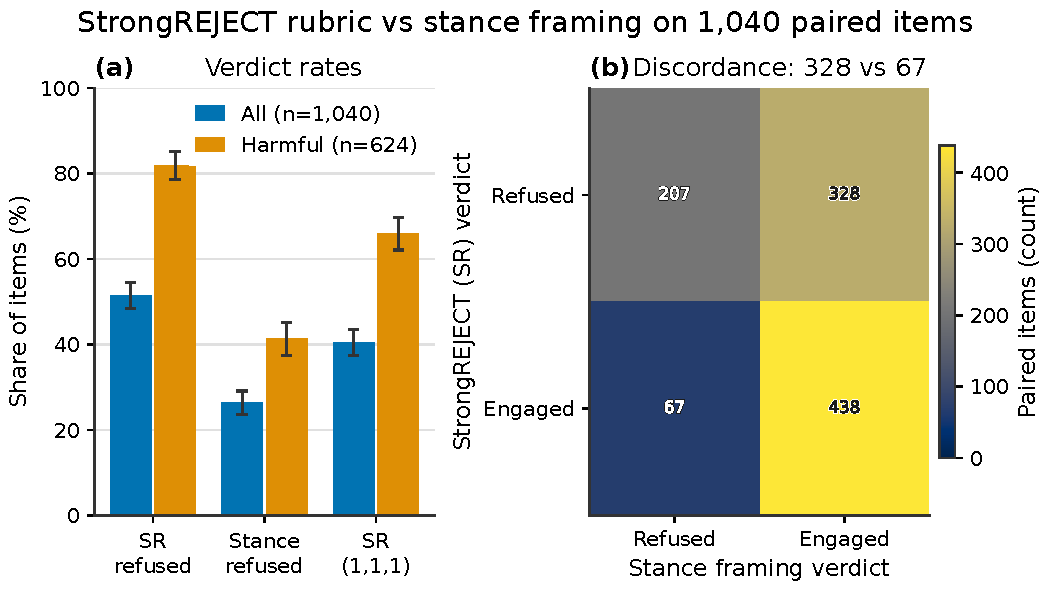
\includegraphics[width=\linewidth,height=0.85\textheight,keepaspectratio]{figures/fig_grader_v0.pdf}
  \caption{Comparison of LLM judge behaviour under the StrongREJECT
  rubric versus stance-based framing on 1,040 paired items. The
  StrongREJECT rubric assigns the degenerate $(1,1,1)$ tuple to 65.9\%
  of harmful items. Of 395 discordant items, 328 are scored as refused by
  StrongREJECT but engaged by the stance framing, versus 67 in the
  opposite direction (McNemar $p < 10^{-42}$).}
  \label{fig:grader}
\end{figure}

\subsection{External Ground Truth}
\label{sec:external}

A census of published safety and capability numbers for the 36-checkpoint
panel (accessed 2026-09-21) finds that 15 of 36 checkpoints have any
published safety number and 5 have an over-refusal number. None appears
on HELM-Safety, AIR-Bench, SALAD, TrustLLM, JailbreakBench or HarmBench.
Open LLM Leaderboard~v2 (OLB2) scores exist for 8 checkpoints.

C2 correlates at $\rho = 0.51$ $[-0.04, 0.91]$ with harm-refusal rate
($n = 23$) and $\rho = 0.69$ with OLB2 average ($n = 8$, descriptive,
$n < 10$). The safety-capability relationship on this panel is negligible:
$\rho(S_2, \text{OLB2}) = 0.24$ $[-0.55, 1.00]$ ($n = 8$), consistent
with the panel's narrow size range and the absence of a general alignment
tax at this scale.

\subsection{The Ceiling: 16 Judged Completions}
\label{sec:ceiling}

The model's own judged behaviour on the SCREEN16 items achieves
$\rho = 0.93$ $[0.75, 0.97]$ with the full CORE-94 target. Given this
16-prompt judged probe, no internal read adds significant information: C2
adds partial $\rho = 0.31$ (one-sided 5\% bound $-0.12$); C12 adds
$-0.01$ (bound $-0.27$). In the reverse direction, given C2, the judged
probe adds partial $\rho = 0.57$ (bound 0.22, significant). An internal
metric that requires no generation and no judge roughly matches the
information in 16 judged completions but has not been shown to exceed it.
The practical advantage is cost: the internal read takes about 16~seconds
per 4B model and requires no LLM judge, versus generating 16 completions
and paying for 16 judge calls.

\subsection{Power and Confounding}
\label{sec:power}

Table~\ref{tab:power} reports the minimum detectable effect at the
realised panel size. At $n = 23$ with $\text{ICC} = 0.103$ across 11
lineages, the design effect is 1.11 and the effective sample size is
20.7, yielding MDE $|\rho| = 0.53$. At $n = 50$ under the same ICC, the
MDE drops to $|\rho| = 0.37$. Every null result in the screen should be
read as ``not detectable at this panel size.''

\begin{table}[!htbp]
\centering
\small
\caption{Minimum detectable $|\rho|$ at 80\% power. ICC and design effect
estimated from lineage-level one-way ANOVA on the balanced target.
$n_{\text{eff}} = n / (1 + (\bar{m} - 1) \cdot \text{ICC})$; MDE
$= \tanh((z_{0.05} + z_{0.20}) / \sqrt{n_{\text{eff}} - 3})$.}
\label{tab:power}
\begin{tabular}{@{}lcccccc@{}}
\toprule
Panel & $n$ & Lineages & ICC & D.E. & $n_{\text{eff}}$ & MDE $|\rho|$ \\
\midrule
Graded (realised) & 23 & 11 & 0.103 & 1.11 & 20.7 & 0.531 \\
Projected & 50 & -- & 0.103 & -- & 44.9 & 0.366 \\
\bottomrule
\end{tabular}
\end{table}

Family identity does not explain the majority of $S_2$ variance on this
panel. The constant-offset control shows that level reads (median relative
change 0.47) and causal reads (0.50) move by comparable amounts under a
constant bias, so the candidates are not invariant to trivial location
shifts.

\paragraph{Confirmation status.}
The 11 frozen Set~A checkpoints have metric values but no safety labels.
Confirmation is \textbf{untested}: no Set~A or Set~B checkpoint has a
balanced label. The frozen survivor hash (SHA-256: \texttt{9f892\ldots})
locks the survivor identity before any confirmation label can be computed.

%% ============================================================
\section{Discussion and Limitations}
\label{sec:discussion}
%% ============================================================

\paragraph{One survivor, narrowly.}
C12 is the sole candidate to pass all six selection rules under their
amended forms, with a partial-$\rho$ bound of 0.006. This margin is
narrow: the bound could move below zero on a modestly different panel.
C12 is significant within two of three large families but not TinyLlama
($\rho = -0.10$, $n = 5$), limiting confidence in cross-family
generality. The confirmation test that would strengthen or disconfirm C12
has not been run.

\paragraph{Rules were amended, not pre-registered in their final form.}
The original S2(b) threshold of 60\% and the original S3 requirement of
all pole checks were too stringent: no candidate passed them. The rules
were amended after iteration-4 results, making the surviving verdicts
exploratory rather than confirmatory in the strict pre-registration sense.
The original and amended verdicts are both reported in
Table~\ref{tab:screen}.

\paragraph{C2: strong correlation, weak independence.}
C2 reaches $\rho = 0.90$, the highest internal-read correlation against a
two-sided target in this study, and clears the amended selection rules.
The detect-versus-grade analysis (Section~\ref{sec:detect}) shows that
about half the panel has $|C2| < 0.1$, indistinguishable from a random
direction, and the rank correlation is partly carried by whether a model
has an ablatable harm direction at all. Within the 10 models where C2
exceeds its null, the restricted $\rho = 0.64$ shows grading ability
beyond detection, but the subsample is small. Furthermore, C2, C2n and
C17 are one measurement, not three.

\paragraph{AMS loses, but the panel is small.}
Every AMS variant correlates worse than C2 and worse than the logit gap,
with a documented padding bug in the reference implementation. The AMS
evaluation in \citet{Messenger2026} used a different panel (14 models,
JailbreakBench compliance, in-sample direction), and the comparison is
between different ground truths. The AMS authors' claim is weaker
(detection and coarse grading at 96 prompts) than ours (rank correlation
with two-sided safety at 16 prompts).

\paragraph{The logit gap remains the floor.}
The first-token logit gap ($\rho = 0.77$) requires no internal access,
costs one forward pass per prompt and fails only S3 (pole control) among
the rules it is eligible for. Any internal metric must justify its
additional complexity against this baseline. C2 significantly exceeds the
logit gap ($\Delta\rho = 0.13$ $[0.01, 0.41]$), but C12 does not
($\Delta\rho = -0.17$ $[-0.47, 0.19]$). The logit gap is blind to
TinyLlama ($\rho = 0.00$), and C2's advantage there ($\rho = 1.00$) is
the strongest argument for internal reads.

\paragraph{Gameability.}
\citet{Muhamed2026} showed that decoy-direction optimisation can mask
abliteration from weight-based detection, and \citet{Burnat2026}
formalise the broader risk that a published safety audit becomes a target
for strategic manipulation once its scoring rule is known. A similar
attack surface exists for C2 and C12: an adversary who knows the harm
direction used in the metric could rotate it without restoring safety. We
did not test adversarial robustness; this is a limitation.

\paragraph{Limitations.}
\begin{itemize}
\item The panel covers only models at or below 4B parameters with
  publicly available safetensors. Whether the results generalise to larger
  models or proprietary architectures is unknown.
\item The prompt set is limited to English single-turn interactions;
  multi-turn and multilingual safety are not tested.
\item C4 and C5 (direction-conditioned weight paths) were not executed.
\item The ROSI reversal is tested on one checkpoint at 128 tokens and two
  checkpoints at 20 tokens.
\item The confirmation test on blind Set~A checkpoints has not been run:
  no safety labels exist for the frozen Set~A models. Until confirmation,
  the screen remains exploratory.
\item The 16-prompt judged behavioural probe ($\rho = 0.93$) remains the
  ceiling. No internal metric adds significant predictive power beyond
  generating and judging 16 completions.
\item Standard safety benchmarks (TrustLLM, AIR-Bench, HELM-Safety) have
  zero coverage on this panel. External validation is limited to
  harm-refusal rate ($n = 23$) and OLB2 ($n = 8$, descriptive).
\end{itemize}

%% ============================================================
\section{Conclusion}
%% ============================================================

We registered 16 candidate cheap safety metrics and executed 14 of them
on 23 chat checkpoints from 8 architecture families against balanced
two-sided ground truth. Under six selection rules (amended after
iteration-4 results showed the original thresholds were unattainable),
one candidate passes: twin d-prime (C12, $\rho = 0.61$), a cross-fitted
measure of harmful-vs-safe separation at the middle layer, clearing the
incremental-signal gate by a margin of 0.006. Self-ablation sensitivity
(C2, $\rho = 0.90$) clears the amended rules but its three surviving
variants are monotone transforms of one measurement, and its correlation
is partly carried by a binary split between models with and without an
ablatable harm direction. The published AMS incumbent
\citep{Messenger2026} correlates worse than both C2 and the first-token
logit gap on this panel, and its reference implementation contains a
right-padding bug. Under the StrongREJECT rubric, LLM judges assign the
degenerate $(1,1,1)$ tuple to 65.9\% of harmful items, with a
328-vs-67 discordance against the stance framing used in this study. No
internal metric adds significant information beyond generating and
judging 16 completions, though the internal read saves generation and
judge cost (about 16~seconds per 4B model, no judge).

The screen's main outputs are methodological: two-sided evaluation with
$S_2$ that penalises blanket refusers, a documented set of failure modes
for 14 internal safety reads, a reusable 23-checkpoint panel, and the
evidence that the simplest baseline, the first-token logit gap, remains
hard to beat. The confirmation test on blind Set~A checkpoints, which
would convert the surviving C12 from an exploratory finding to a
validated metric, remains the priority for future work.

\bibliographystyle{plainnat}
\bibliography{references}

\end{document}
